% !TEX encoding = UTF-8
% !TEX TS-program = pdflatex
% !TEX root = computabilità e algoritmi.tex
% !TEX spellcheck = it-IT
\section{Sweeping}\label{sweeping}

C'è un insieme di segmenti nel piano e ci chiediamo se tra questi ce ne sono almeno due che si intersecano. Non interessa sapere quanti o quali sono, basta poter dire che ci sono o non ci sono.

Con l'approccio naive che prova a due a due i segmenti si ottiene una complessità pari a $O(n^{2})$, mentre con opportuni accorgimenti è possibile rispondere in $O(n \log n)$.

Da notare che per trovare \textbf{tutte} le intersezioni non si può scendere sotto $O(n^{2})$ perché è necessario provare tutte le coppie di segmenti.

L'algoritmo si basa sull'utilizzo di una retta che funziona da spazzola e che viene utilizzata per scansionare i vari segmenti.

Dato che la retta si sposta da sinistra a destra, questa retta incontrerà per primo l'estremo sinistro e lascerà il segmento tramite l'estremo destro.

La prima operazione da fare è quindi l'ordinamento dell'array contenente tutti i segmenti, in modo che il primo elemento sia quello con l'estremo sinistro più a sinistra. 
Come tie-breaking per i segmenti con l'estremo sinistro e quello destro uguali, viene messo per primo quello con coordinata \emph{y} minore. 
Lo stesso vale anche se due segmenti hanno l'estremo sinistro con la stessa \emph{x}.

Lo spostamento della retta non deve essere necessariamente continuo, basta che si sposti sui vari estremi dei segmenti. 
Quando la retta si sposta su un estremo prende il nome di \textbf{evento} pertanto, durante l'esecuzione dell'algoritmo ci sono \emph{2n} eventi.

Ogni evento può essere rappresentato da una coppia contenente le informazioni riguardante il segmento e un booleano che specifica se è l'estremo destro o l'estremo sinistro.

Tutti gli eventi vengono poi raccolti in un array ordinato per \emph{x} crescente, facendo in modo che gli eventi relativi agli estremi sinistri vengano prima di quelli relativi agli estremi destri. 
Questo per gestire le situazioni in cui l'estremo sinistro di un segmento coincida con un estremo destro di un altro segmento.

$$
e_1 \leq e_2 = \textsc{True} \Leftrightarrow \begin{cases}
x_1 < x_2  \text{ oppure }\\
x_1 = x_2 \text{ e } e_1.left = \textsc{True} \text{ e } e_2.left = \textsc{False} \text{ oppure} \\
x_1 = x_2 \text{ e } e_1.left = e_2.left \text{ e } y_1 \leq y_2
\end{cases}
$$

La cosa importante è che l'ordinamento definito sugli eventi sia totale perché questi devono essere poi ordinati utilizzando un algoritmo di ordinamento. 
Dal momento che il test dell'ordine richiede tempo costante, l'ordinamento degli eventi può essere fatto in $O(n \log n)$.

Per mantenere le informazioni riguardanti i segmenti intersecati dalla spazzola viene utilizzata una struttura dati \emph{T} che prende il nome di \textbf{stato della spazzola} la quale contiene tutti i segmenti intersecati da essa.

Lo stato della spazzola tiene i segmenti ordinati secondo la coordinata \emph{y} con la quale intersecano la spazzola. 
Per i segmenti verticali viene scelto l'estremo inferiore.

Quando la spazzola viene spostata l'ordine dei segmenti presenti nello stato potrebbe cambiare, ma questo può succedere solamente se tra un evento e l'altro c'è un'intersezione, pertanto l'algoritmo deve evitare di fare spostamenti della spazzola oltre il punto di intersezione.

Per modificare lo stato della spazzola è possibile utilizzare:

\begin{itemize}
\item
  \textsc{Insert($T,s$)} che aggiunge un segmento \emph{s} alla struttura dati, rispettando l'ordinamento.
\item
  \textsc{Delete($T,s$)} che rimuove il segmento \emph{s} dalla strutta dati.
\item
  \textsc{Below($T,s$)} che restituisce il segmento \emph{s'} che precede \emph{s} nell'ordinamento considerato e che ritorna \textsc{Nil} quanto \emph{s} è il primo
\item
  \textsc{Above($T,s$)} che restituisce il segmento \emph{s'} che segue \emph{s} nell'ordinamento considerato e che ritorna \textsc{Nil} se \emph{s} è l'ultimo.
\end{itemize}

Per implementare \emph{T} è possibile utilizzare un albero rosso-nero il quale permette di effettuare tutte le operazioni in tempo $O(\log n)$.

Se due segmenti si intersecano si troveranno per forza contemporaneamente nello stato della spazzola. 
Però comunque controllare tutte le coppie di segmenti richiederebbe $O(n^{2})$ pertanto l'algoritmo si limita a controllare ogni segmento con quello precedente e quello successivo.

Inoltre, tra un'evento $e_1$ e il successivo $e_2$, l'ordine dei due segmenti $s'$ e $s''$ cambia soltanto se i due segmenti segmenti si intersecano in un punto di coordinata $x$ compresa tra $x_1$ e $x_2$

\begin{figure}[htbp]
	\centering
	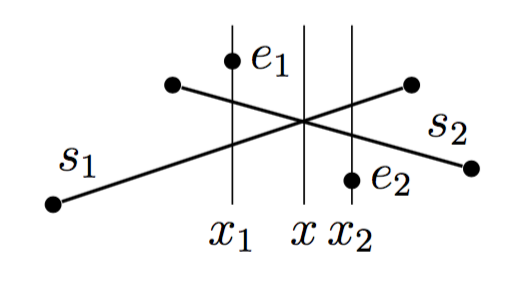
\includegraphics[width=0.3\textwidth]{./notes/immagini/l31-fig23.png}
\end{figure}

Assumendo che non siano ancora stati trovati dei segmenti che si intersecano, quanto si verifica un nuovo evento questo può essere associato ad un estremo sinistro o destro.

Se l'evento è sinistro, basta controllare che il nuovo segmento non si intersechi con il precedente e successivo. 
Se invece è un evento destro basta controllare che i due segmenti che diventano consecutivi non si intersechino. 
Il controllo dell'intersezione è già stato affrontato e viene fatto in tempo costante.

\begin{breakablealgorithm}
	\caption{\textsc{Any-Segment-Intersect}: intersezioni in un insieme di segmenti}
	\begin{algorithmic}[1]
		\Function{Any-Segment-Intersect}{$S$} 
		    \State // $S$ insieme di $n$ segmenti
		    \State // Ordina gli estremi dei segmenti $s_i = (p_i,q_i)$ in modo che $p_i$ sia l'estremo sinistro
		    \State // Costruisci la sequenza degli eventi $e_1 \ldots e_{2n}$
		    \State // Ordina la sequenza di eventi come precedentemente definito
		    \For{$i = 1 \textbf{ to } 2n$}
		        \State $s \gets e_1.s$
		        \If{$e_i.left$}
		            \State \textsc{Insert}$(T,s)$
		            \State $s' \gets \textsc{Above}(T,s)$
		            \If{$s' \neq \textsc{ Nil } \textbf{ and } \textsc{Segment-Intersect}(s,s')$}
		                \State \Return \textsc{True}
		            \EndIf
		            \State $s'' \gets \textsc{Below}(T,s)$
		            \If{$s'' \neq \textsc{ Nil } \textbf{ and } \textsc{Segment-Intersect}(s,s'')$}
		                \State \Return \textsc{True}
		            \EndIf
		        \Else \Comment{Estremo destro}
		            \State $s' \gets \textsc{Above}(T,s)$ \Comment{prima li cerco e poi tolgo $s$}
		            \State $s'' \gets \textsc{Below}(T,s)$
		            \If{$s' \neq \textsc{Nil} \textbf{ and } s'' \neq \textsc{Nil} \textbf{ and } \textsc{Segment-Intersect}(s',s'')$}
		                \State \Return \textsc{True}
		            \EndIf
		            \State \textsc{Delete}$(T,s)$
		        \EndIf
		    \EndFor
		\State \Return \textsc{False}
		\EndFunction

\end{algorithmic}
\end{breakablealgorithm}

È semplice dimostrare che l'algoritmo ritorna \textsc{True} se ci sono due segmenti che si intersecano.

Risulta però più difficile dimostrare che quando l'algoritmo ritorna \textsc{False} nessun segmento si intersechi. 
Ovvero che se c'è un'intersezione allora l'algoritmo ritorna \textsc{True}.

Assumiamo quindi che ci siano una o più intersezioni, e tra tutte prendiamo quella con la coordinata del punto d'intersezione $x_p$ più a sinistra con tie-break $y_p$ più basso.

Consideriamo quindi l'evento in cui viene inserito l'ultimo segmento che si interseca nel punto $x_p$. 
Sia \emph{s} il segmento che viene inserito e \emph{s'} il segmento con cui \emph{s} si interseca. 

Se \emph{s} e \emph{s'} sono consecutivi, viene fatto il test e l'intersezione viene correttamente rilevata. 

Se invece non sono consecutivi esiste un segmento \emph{s''} che, nello stato della spazzola, si trova tra \emph{s} e \emph{s'}. 

\begin{figure}[htbp]
	\centering
	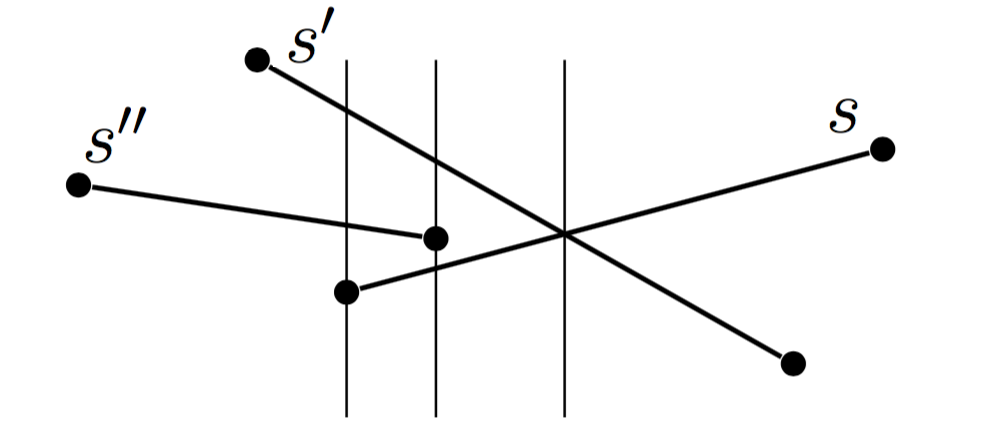
\includegraphics[width=0.4\textwidth]{./notes/immagini/l31-fig1.png}
\end{figure}

Questo segmento deve terminare prima di incontrare il punto di intersezione, perché altrimenti dovrebbe intersecare \emph{s} o \emph{s'} prima di $x_p$ e questo è assurdo per ipotesi. 
Si ha quindi che prima di trovare $x_p$ si verificherà l'evento destro di \emph{s''} che renderà consecutivi \emph{s} e \emph{s'} e anche in questo caso l'intersezione viene rilevata. 
Lo stesso discorso vale se ci sono più segmenti tra \emph{s} e \emph{s'}.

Da notare che quando viene inserito \emph{s} all'interno della spazzola possono essere già presenti altri segmenti che si intersecano tra loro, ma che hanno un punto di intersezione maggiore di $x_p$.

(C'è anche da dimostrare che la spazzola non supera mai un'intersezione, ma questo segue da quanto appena dimostrato, perché abbiamo visto che la spazzola è in grado di rilevare correttamente la prima intersezione ed una volta che l'ha rilevata, l'esecuzione dell'algoritmo termina)

Per quanto riguarda la \textbf{complessità} il tempo di esecuzione dell'algoritmo è $O(n)$ per costruire la sequenza degli eventi, $O(n \log n)$ per ordinarli e infine $O(n)$ per esaminarli nel ciclo \texttt{for}. 
In totale tempo $O(n \log n)$.

\subsection{Intersezione con la spazzola}

\textit{\textbf{Esercizio 9}} \todo{Verificare correttezza}

Abbiamo detto che se lo stato della spazzola viene rappresentato con un albero rosso-nero le quattro operazioni possono essere eseguite in tempo logaritmico.
Questo è vero soltanto se riusciamo ad effettuare in tempo costante il test su quale tra i due segmenti ha l'intersezione più alta con la retta della spazzola.

L'algoritmo riportato, dati due segmenti $s = (p_1,p_2)$, $s' = (p_3, p_4)$ e la coordinata \textit{x} della spazzola, ritorna \textsc{True} in tempo costante se $s$ precede $s'$ nella spazzola.

\begin{breakablealgorithm}
	\begin{algorithmic}[1]
		\Function{Segments-Prec}{$p_1,p_2,p_3,p_4$}
			\If{$x_1 = x_3$}
				\State \Return $y_1 \leq y_3$ \Comment{stessa \textit{x}, viene prima quello più basso}
			\EndIf
			\If{$x_1 > x_3$}
				\State $d_1 \gets \textsc{Angle-Left}(p_3,p_4,p_1)$
				\State \Return $d_1 \leq 0$
			\Else \Comment{$x_1 < x_3$}
				\State $d_2 \gets \textsc{Angle-Left}(p_1,p_2,p_3)$
				\State \Return $d_2 \geq 0$
			\EndIf
		\EndFunction
	\end{algorithmic}
\end{breakablealgorithm}

Se $p_1$ coincide con $p_3$ l'ordine perde di importanza perché è un punto di intersezione e all'algoritmo della spazzola non interessa quello che succede dopo un punto di intersezione.

Se invece $x_1$ viene dopo di $x_3$ mi basta osservare se $p_1$ si trova a destra o a sinistra del segmento $s' = (p_3,p_4)$. 
Da notare che se l'angolo è 0, si ha che $p_1$ appartiene al segmento $(p_3,p_4)$ e quindi è un punto di intersezione, quindi posso considerare i due segmenti coincidenti e ritornare 0 va bene. L'altro caso è simmetrico.

Il tutto funziona perché vengono sempre testati due segmenti comparabili, ovvero che vengono intersecati contemporaneamente dalla spazzola e perché dopo il punto di intersezione l'ordinamento perde di importanza.

\subsection{Estensioni dell'algoritmo}

\subsubsection{Verifica della semplicità di un poligono}

\textit{\textbf{Esercizio 10 e 11}}

Si vuole trovare un algoritmo per decidere in tempo $O(n \log n)$ se un poligono di \emph{n} vertici è \textbf{semplice}, ovvero se i lati del poligono non si intersecano.

Per fare ciò basta modificare in \textsc{Any-Segment-Intersect} in modo che quando rileva un'intersezione verifichi che questa sia tra estremi gli estremi dei segmenti che delimitano e se questo è vero non la segnali e continui la ricerca. 

C'è un possibile problema perché l'algoritmo continua dopo un punto di intersezione, il che non era previsto quando è stata dimostrata la correttezza.

Bisogna quindi dimostrare che l'ordinamento della spazzola rimane corretto anche dopo un punto di intersezione.

Se almeno uno dei due è un estremo destro, un segmento viene tolto e quindi non ci sono problemi. 

Se invece sono entrambi estremi sinistri è necessario garantire che l'ordine della spazzola rimanga corretto, ovvero è necessario modificare \textsc{Segment-Prec} in modo che se $x_1=x_3$ e $y_1=y_3$ tenga in considerazione anche la posizione degli estremi destri per stabilire quale dei due segmenti sta sotto.

Questa modifica può essere estesa anche alla verifica se due poligoni semplici si intersecano tra loro, basta non segnalare le intersezioni tra i segmenti appartenenti allo stesso poligono.

\subsection{Intersezione di cerchi}

\textbf{\textit{Esercizio 12}} \todo{Completare}

Dati $n$ cerchi $c_1, \ldots c_n$ nel piano, per ognuno dei quali sono note le coordinate del centro e la dimensione del raggio.
Stabilire in $O(n \log n)$ se ci sono dei cerchi che si intersecano.

Due cerchi si intersecano se la distanza tra i due raggi è minore della somma dei due raggi, la quale può essere calcolata anche senza ricorrere alla radice quadrata.

Se per ogni cerchio viene preso in considerazione il diametro orizzontale, si può riutilizzare lo stesso algoritmo con un test d'intersezione diverso che verifica se la distanza tra i due centri è maggiore della somma dei due raggi.
